\section{Result}
This section covers the results of this project. It will explain, how the final workflow works and what kind of product were produced during the time of this bachelor thesis.

\subsection{Discussion}
\label{sub:Discussion}
In this section we will discuss all the results shown in the implementation. It will highlight the algorithms used and then conclude with a comparison of our results to the other works mentioned "Introduction" under "Similar works".

\subsubsection{Door detection}
The machine learning approach, called "Cascade classifier", for door detection shows good results. Most doors on the floor plans can be detected. On all plans the F1-Score was at least at 75 percent. This was good enough for a good implementation of the gap closing algorithm. Another important notice is, that cleaned floor plans show an improvement in detection rate of the F1-score up to a 100 percent. This shows that with little effort the detection can work at very high rates. All of these results can be found in figure~\ref{fig:CCF1ScoreGraph}. What is also shown with this graph is, that the detection rate can be further improved if better or more training images can be found. Almost every training we did showed improvements and with more time it is likely to create a better cascade file and let this trend continue.

\subsubsection{Door closing}
The door closing algorithm based on the door detection algorithm shows very good results as well. As seen in figure~\ref{fig:simpleDoorClosing}, the door closing algorithm works in most cases very well. The F1-Score is for all but one image above 75 percent. Very important here is the Recall, it is on more than half of the images at a 100 percent. This means that all doors on the plan are closed. The low precision is due to the fact that some windows are also recognized as doors, therefore the plan has quite a few false positives. It is important to remark, that this algorithm handles false positives very well. In most cases the detection of a false positive will not lead to a negative effect, as it just draws over a wall. A further description of this problem is found in section~\ref{sec:DoorClosingComparison}.

\subsubsection{Room detection}
The room detection done based on all this preprocessing, shows results above 80 percent for the F1-Score on all of the cleaned up plans. As explained in section~\ref{sec:ConnectedComponents}, the uncleaned versions have problem with the outer wall closing and most of them show terrible results with room detection. All of these results are based on the fact, that no post processing from the user was done. The exact values can be found in figure~\ref{fig:RoomDDResult}. What improved the room detection by a lot was the user interaction as show in figure~\ref{fig:RoomDDEResult}. On all plans, the F1-Score is above 80 percent, most of them are even on a 100 percent. With enough user interaction, all scores can be on a 100 percent, as the user can basically fully redraw the floor plan to an optimal one for detection. This graph represents tests with user interaction. The time used is comparable to that what user a user would take if the program would be used in a working environment.

\subsubsection{Other works}
Compared to the works of Mace, Valveny,Loctea and Tabbone \citep{mace_valveny_loctea_tabbone_2010} and Ahmed,Liwicki,Weber and Dengel \citep{ahmed_liwicki_weber_dengel_2012}, this work shows some improvement. Our algorithm shows an average of 83.8 percent of room detection accuracy on cleaned up plans. This is slightly above the 82 percent that Ahmed,Liwicki,Weber and Dengel showed. It is an bigger improvement if you compare it to their 79 percent, which was the same algorithm but without combining rooms based on room labels. It is a big step compared to the 69 percent detection accuracy achieved by Mace, Valveny,Loctea and Tabbone. Generally can be said, that uncleaned floor plans will achieve a detection accuracy still below 40 percent, as there is just too much noise that can not be canceled. But simple floor plans or little pre-cleaning can boost the detection rate of those algorithms in the higher 90 percent without additional user input. 

\subsubsection{Improvements}
The comparison in figures \ref{fig:ClicksPerPlan} and \ref{fig:TimePerPlan} show the improvement that the automated algorithm shows compared to what is used at the PlanfabrikGmbH. The graphs show that the time and clicks used for analyzing the plans with the algorithm show about the same no matter how big or complicated the plan is. This is contrary to the current approach, which takes more time and clicks with more difficult plans. Generally can be said that time and clicks used are less when using the new algorithm. But the time and effort saved is better the more complicated a plan is. 

\subsection{Workflow}
\label{sub:FinalWorkflow}
During the time of this project, we tried out different algorithms and processes (Section~\ref{sub:Discussion}), to create a workflow, which solves the stated task (Section~\ref{sub:ProblemDescription}).

\begin{figure}[H]
	\centering
	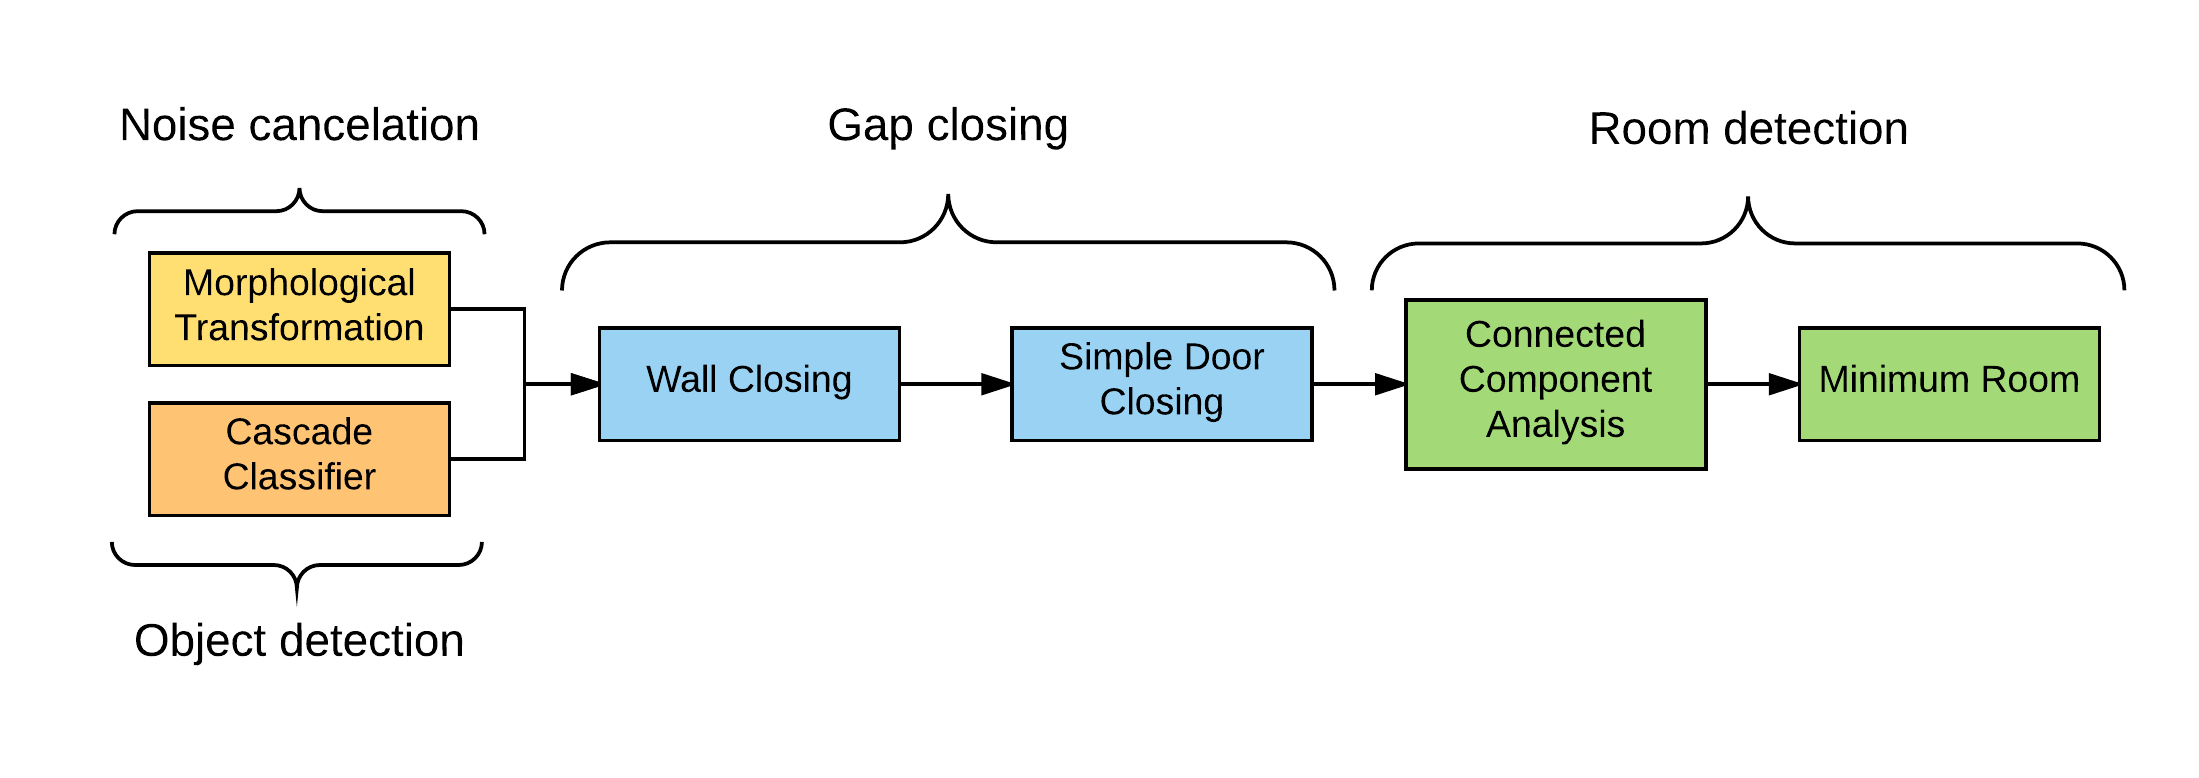
\includegraphics[width=1.0\textwidth]{FinalWorkflow}
	\caption{Final workflow flowchart.}
	\label{fig:FinalWorkflow}
\end{figure}

The workflow is visualised in figure~\ref{fig:FinalWorkflow} is the same workflow as the workflow three, described in section~\ref{sub:workflow3}.

It starts with the object detection (Section~\ref{sub:ObjectDetection}), which detects all doors on a floor plan. This information is saved into the meta image format (Section~\ref{sub:MetaFormat}) for further processing. Then the noise cancelation (Section~\ref{sub:NoiseRemoval}) removes noise like furniture, markings and other elements on the plan, to create a skeleton of the building walls.

Due the fact, that the noise cancelation removes also the windows of the building, the wall closing algorithm (Section~\ref{sub:WallClosing}) finds the outer contour and closes the gaps. Together with the information gathered in the objection detection step, the simple door closing algorithm (Section~\ref{sub:SimpleDoorClosing}) closes the gaps between the walls, where the doors should be.

After the cleanup and reconstruction process, the room detection is processed (Section~\ref{sub:RoomDetection}). As final step, the minimum room detection (Section~\ref{sub:MinimumRoom}) filters out rooms, which are too small, in relation to the average room size.


\subsection{Prototype}
To create a user friendly application, we implemented a user interface prototype (Section~\ref{sub:userInterface}), which supports the execution of the workflow described in section~\ref{sub:FinalWorkflow}.

\begin{figure}[H]
	\centering
	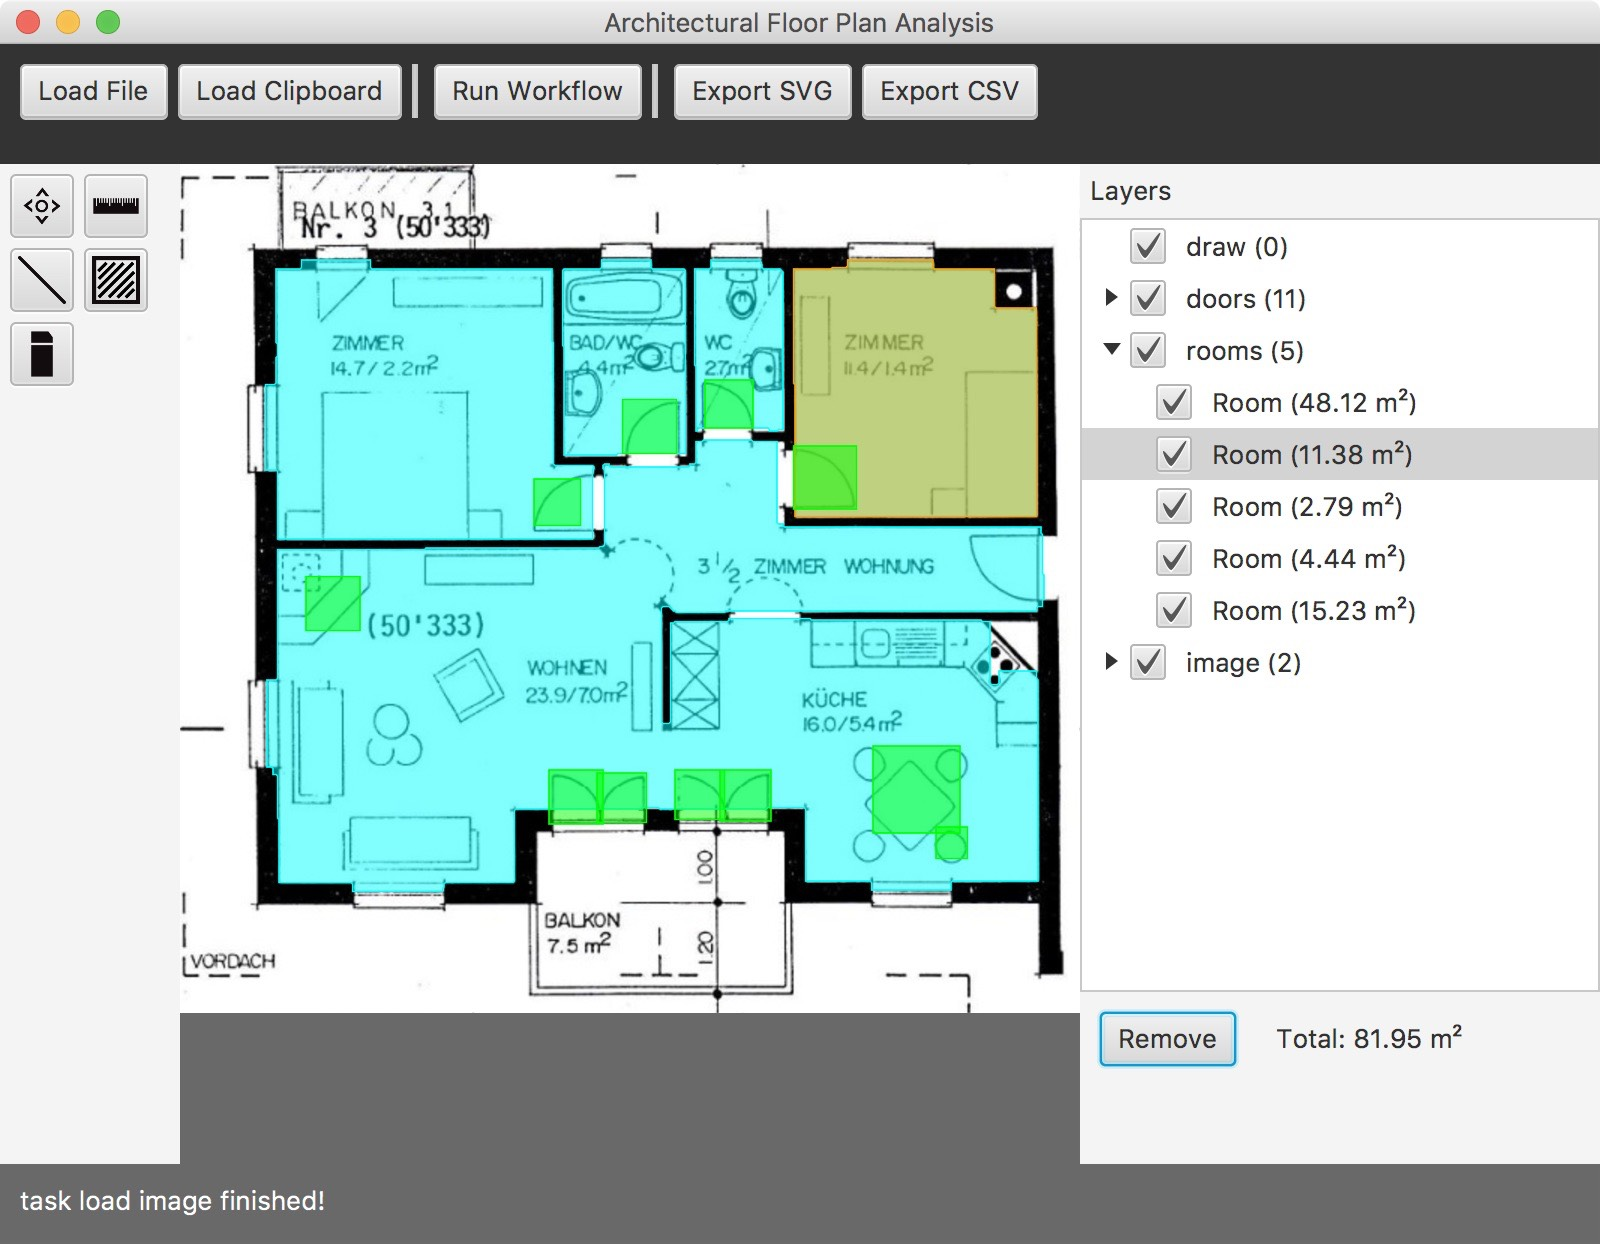
\includegraphics[width=1.0\textwidth]{UserInterfacePrototype}
	\caption{A screenshot of the user interface prototype at the end of the detection process.}
	\label{fig:UserInterfacePrototype}
\end{figure}

The prototype is able to load floor plans and run the predefined workflow. With editing tool, the user is able to make enhancements between each step and can fix errors or mistakes of the algorithms.

After processing, the software supports analysing the result and directly receive the size of each room. For further processing of the results, the software is capable of exporting the rooms either into SVG or CSV (Section~\ref{sub:ImportExport}).

\subsection{Limitations and restrictions}
The current algorithm is able to analyse floor plans and detect various objects on it. But there are some preconditions. which have to be fulfilled, to ensure a smooth process.

First of all, the plan has to be in a raster image format. Currently the software is not able to read DXF or DWG plans, so the user have to convert the floor plans manually. Another problem connected with this restriction is, that the export of the results, is limited to CSV and SVG files (Section~\ref{sub:ImportExport}).

Another limitation is, that the noise cancelation (Section~\ref{sub:NoiseRemoval}) needs thick walls to detect the right skeleton of the building. If the walls are too thin, they will be detected as noise and removed. The advantage of this limitation is, that we did not to use a heuristic to detect the rooms, which would limit the room polygon to a specific shape. We are able to detect a room of any shape.

To detect the outer contour of the building, it is necessary to have a noise free plan. No object should be on the outer side of the building. We tried to solve this limitation with an morphological opening and a polygon approximation of the contour, but it is still recommended to have a clean plan. Otherwise the outer wall will not be closed correctly and windows will stay open.

The fact, that the user has to set the right parameters for each algorithm, is a big limitation. With live preview and help texts, we tried to make this as comfortable as possible for the user.

